\documentclass{article}
\usepackage[utf8]{inputenc}
\usepackage{graphicx}
\newcommand{\source}[1]{\hfill Source: {#1}} %command definition for sources in figures


\title{Evaluating global air pollution models using air quality sensors onboard a carrier bicycle in the Netherlands}
\author{Meng Lu et al. }
\date{March 2020}

\begin{document}

\maketitle

\section{Introduction}
Chronic exposure to air pollution poses a threat to public health. World Health Organization estimated that air pollution has contributed to 7 million deaths in 2016 [1]. From a medical perspective, common air pollutants such as particle matters and nitrogen oxides (NO$_2$) damage the cardiovascular and respiratory systems [3-4]. Air pollution mapping is crucial for interventions to abate exposures. Multiple factors influence the concentration of air pollution. In the Netherlands, specifically, road traffic produces most NO$_2$ pollution [8]. Emissions from traffic can be direct and indirect. Atmospheric NO$_2$ is mostly an indirect secondary emission as an oxidation result of emitted NO, while the direct primary emission as NO$_2$ is minor [9]. Apart from traffic conditions, topography and tropospheric processes both can also contribute to NO$_2$.
\par
Extensive research has mapped air pollution concentration using ground monitor station observations, satellite measurements, and ancillary NO$_2$ data (commonly called predictors, including all the variables relating to the emitting and dispersing processes of NO$_2$ such as climate, land cover, traffic network)[13,14,15]. Ground monitors can be routinely run or are project-oriented, which requires extra cost, mainly when other attributes such as temperature and wind direction are recorded [16]. Recent studies show a rise in low-cost ground sensors [17, 18, 19], but their study-specific conditions constrain generalization for larger areas. As for satellites, their coverage range is more extensive than regional monitor networks at a higher cost [16]. The target is different for ground monitors and satellites: the satellite records the column from the ground to the stratosphere, while the ground monitor takes the near-surface concentration, which is more relevant to human health [16]. This discrepancy may cause different results for exposure measurement given the same study area. 
\par
Based on the measurement input, air pollution mapping methods has three major genres, which can be combined in some cases. The first genre, named interpolation, derives spatially continuous pollution concentration levels from point records. Typical approaches include Kriging and the Inverse weighted distance method [20, 21]. The second genre, the dispersion model, focuses on the atmospheric process of pollutants. It takes into account the dynamics of mass transport, turbulence, and chemical transformation [22]. The third genre, called Land Use Regression models is in use widely in epidemiological studies to calculate pollution map for exposure assessment [23]. This approach assumes that the air pollution level relates to geographic attributes. Frequent empirical attributes concern population, traffic, land cover, transportation accessibility [16]. 
\par
To map air pollution globally, regression-based methods and machine learning algorithms are in use widely. They gain prediction power from unique calculation processes, and in practise they can combine the aforementioned three genres to some degree.
\par
Several studies compared regression-based and machine learning models to map air pollution to pinpoint their strengths and constraints. \cite{chen2019comparison, kerckhoffs2019performance, adam2014spatiotemporal, DEHOOGH2014382} compared different geostatistical-based, linear regression-based and machine learning-based techniques in air pollution mapping. \cite{chen2019comparison, kerckhoffs2019performance} both found similar cross-validation accuracy between machine learning-based techniques, as well as between ensemble tree-based techniques and regularized linear regression. Therefore, they concluded there is no difference in performance between these methods, but neither \cite{chen2019comparison} or\cite{kerckhoffs2019performance} show spatial prediction patterns of the different models. The question is: do the similar prediction accuracy obtained from different models indicate the same performance? In the global NO$_2$ modeling study of Lu2020, it is found that various ensemble tree-based methods obtained almost the same cross-validation accuracy can predicted very different spatial patterns. This calls for a re-evaluation of different ensemble tree-based methods using additional ground validation data to further understand different models and to imply a validation method that accounts for spatial prediction patterns. 

\par
In this study, we address this pressing need  We used a mobile air quality station on board a cargo bike to monitor selected air pollutants (called “cargo-bike”). The bicycle covered a selected area close to the routes followed by the Four Days Marches in Nijmingen, the Netherlands.  From July 16 to 19, 2019. The cargo-bike measures NO$_2$ twice a day, with the same route taken for all the measurements.  

\par
The goal of this study is to re-evaluate various linear regression and machine learning-based air pollution models, particularly regularized regression, Lasso, and emsemble tree-based methods: Random Forest (RF) and XGBoost (XGB). In addition, despite the temporal mismatch, we compared the global air pollution model, which is made for 2017 and available for the daytime  (7 am – 10 pm local time), with the cargo-bike measurements to understand the amount of spatial variability that an annual global model could explain at the local time.  

\section{Data and Methods}
\subsection{Cargo-bike measurements}
The cargo-bike and the instruments onboard weights 160 kg. It carries a 150 WP solar panel and can work 3 – 5 hours continuously.  Due to the weather, the measurements in the afternoon have severe deficiencies and are therefore not used in this study. In the morning, the measurements are taken from 8 - 11am. 
[detailed description to be added by TNO].
The cargo-bike measurements averaged over the four days have the mean of 11.21 ug/m3. 
\begin{figure}
    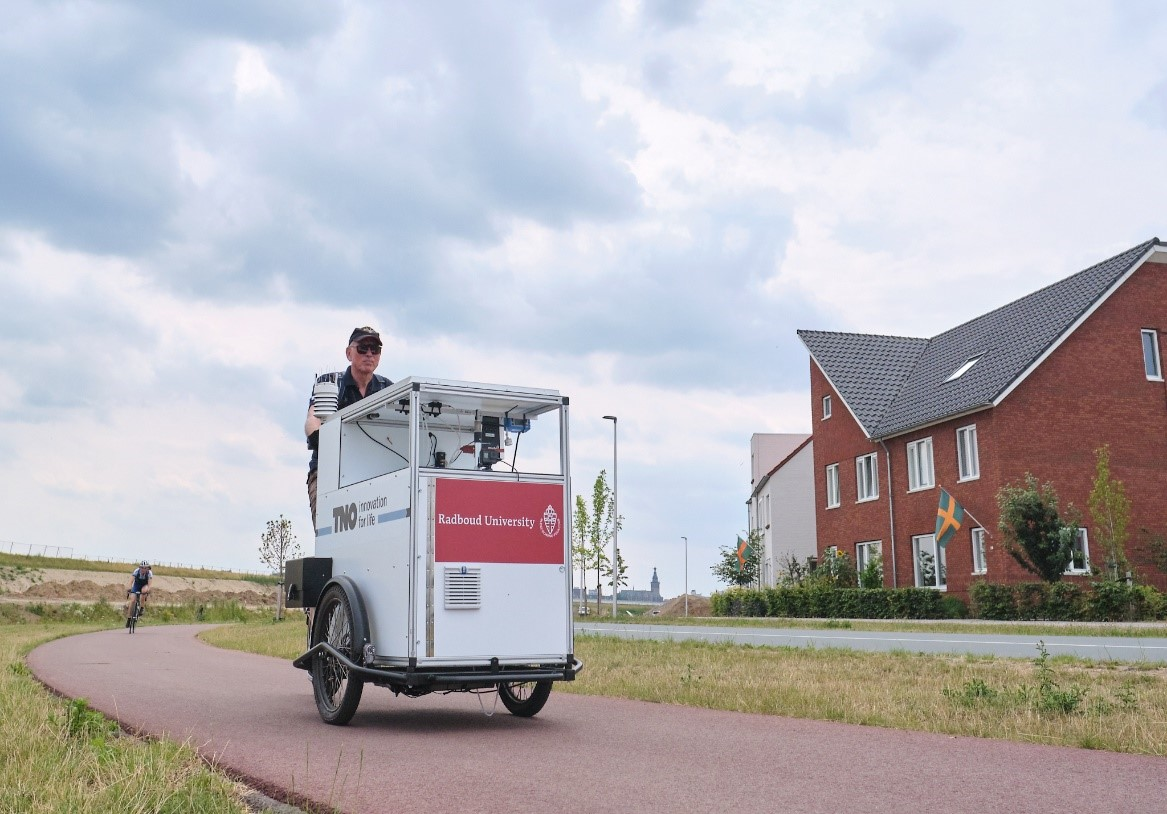
\includegraphics[width=\linewidth]{f1a.jpg}
    \label{bike}
    \caption {bikefits}
\end{figure}
\begin{figure}
    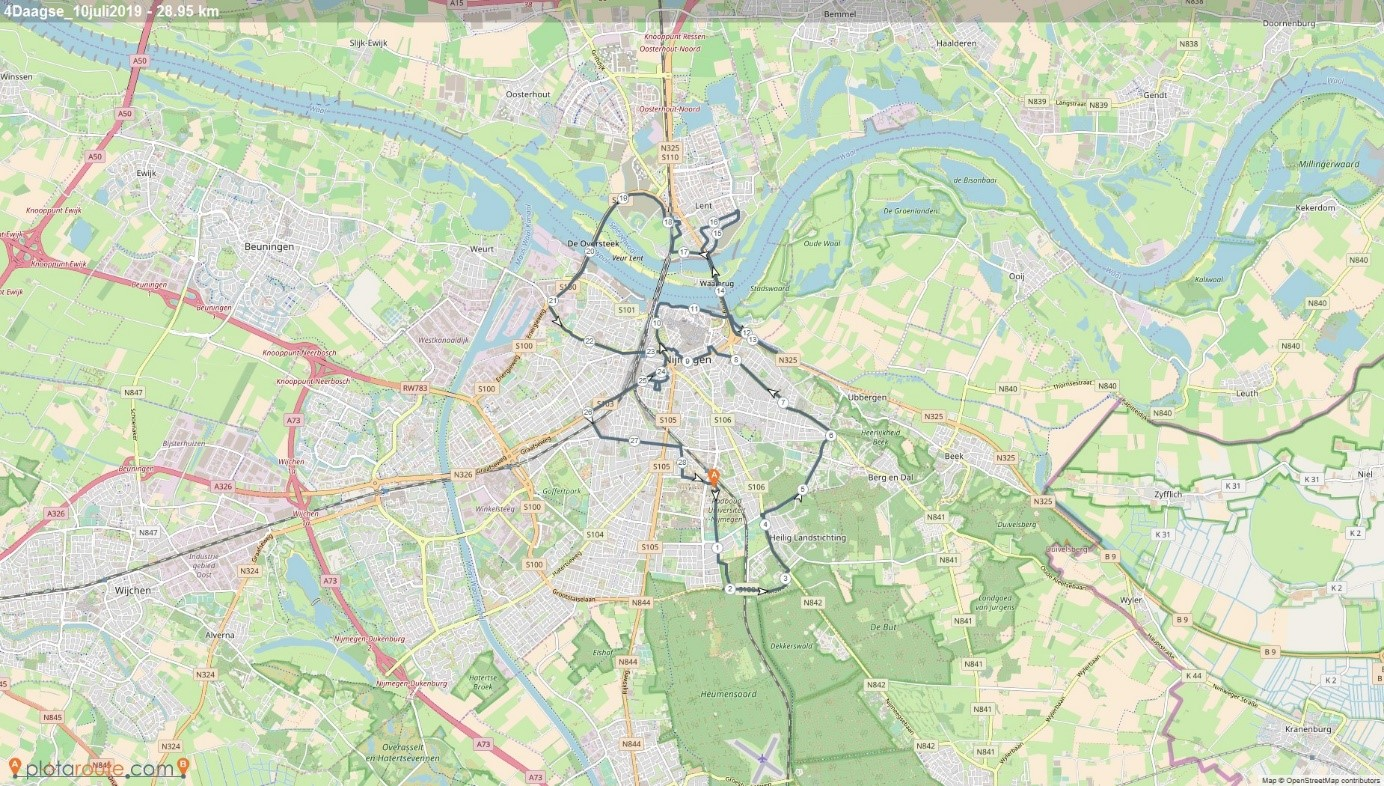
\includegraphics[width=\linewidth]{f1b.jpg}
    \label{route}
    \caption {routes taken by the cargo-bike on openstreetmap[cite]. “A” indicates the starting point.The point numbers indicated on the map are used to indicate the routes. For example route from point 1 to point 2, which is called route 1-2 in this study.}
\end{figure}


\subsection{Ground monitor stations in Netherlands and Germany}

Since the Netherlands (41,543 $km^2$) contains only 77 stations, we also incorporated the ground monitor network from Germany (357.386 $km^2$) to study if the strength can be borrowed to improve the modelling accuracy. The ground monitoring stations data are from European Environment Agency (cite) for the Netherlands and the Umwelt Bundesamt (cite) for Germany. Stations with inadequate data such as  missing value at certain hours are neglected. The measurements of the same time span as the Cargo-bike measurements are used.  


\subsection{Ground monitor stations in Nijmingen}
the ground measurements are gathered from two LML stations, one is the Nijmegen-Graafseweg station (called Graafseweg station, Latitude: 51.941372, Longitude 5.857777). The other is Nijmegen-Ruyterstraat station (called Ruyterstraat station, Latitude: 51.838221, Longitude: 5. 856938). The station is managed by RIVM to monitor air pollution from local traffic. The measurements averaged over the same periods of cargo-bike is 23.25 ug/m3 at Graafseweg and 14.03 ug/m3 at Ruyterstraat.
\par
The openaq data is used for the global model predictions (see Lu et al. 2020). Three methods are evaluated in this study, namely xgboost, random forest, and Lasso. 



\par
%We used all the ground monitoring stations in the airbase[cite] for the whole Europe and evaluate the models at 3 scales: 1) Europe-wide (using all the ground station measurements), 2) Netherlands and its neighbouring countries, Germany, France, Belgium, 3) Netherlands. 
\par
We firstly use geographically weighted regression to explore local stationaries, and compare three types of spatial prediction methods: 1) Gaussian process, which include Kriging and cokriging, 2) regression- based, which include Lasso and ElasticNet, and 3) machine learning based, which include random forest and xgboost. These methods are selected as they are representative to the current spatial prediction techniques.  


\subsection{Global NO$_2$ models}
Based on hyperparameter setting recommendations provided by Lu et al (2020) We used 1000 trees for all the methods. The maximum tree depth for xgboost is set to 6 and learning rate set to 0.02. Other settings are the same as Lu et al (2020). As the global model predictions are for entire year, we scale them to the same timespan as the cargo-bike measurements by multiplying the predictions to the ratio between the global model prediction and the LML measurements averaged over the timespan of the cargo-bike measurements (July 16 -19, 8 am - 11 am), which means after scaling, the mean of the xgboost, random forest, and Lasso predictions are also 23.25 ug/m3 if scaled using the Graafseweg station and 14.03 if scaled using the Ruyterstraat station.   


\subsection{Separating between background and traffic areas}
To validate the predictions close to roads and faraway from roads, we made two groups. If the location is within 500 m distance away from the primary roads, they are grouped into traffic areas, if the location is farther away from the primary roads, they are grouped into background areas. Figure X shows the cargo-bike routes that are in traffic areas and background areas. 
separating between traffic and background areas, cargo-bike measurements.
\begin{figure}
    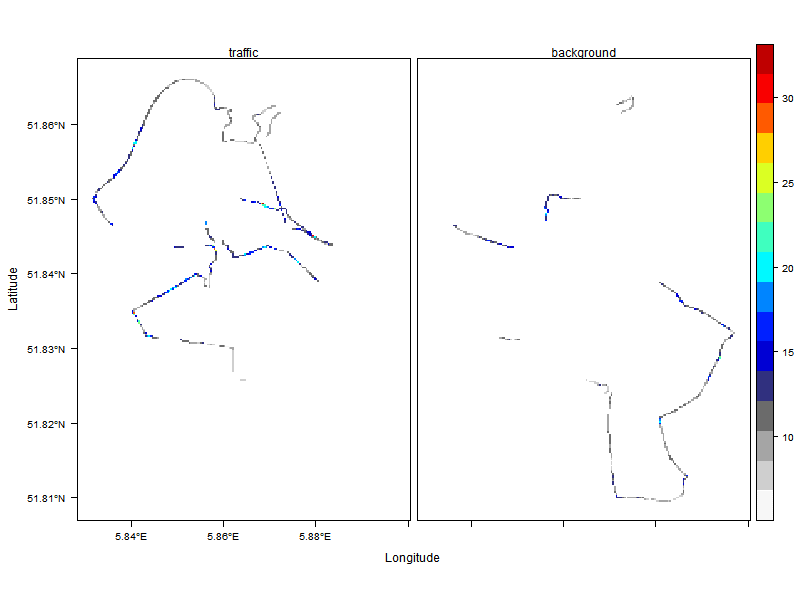
\includegraphics[width=\linewidth]{f2.png}
    \label{seperate}
    \caption {separating between traffic and background areas, cargo-bike measurements.}
\end{figure}


\section{Result}
\subsection{Variable importance}

\begin{table}[!htbp] \centering 
  \caption{Ranking of the top 20 important variables of XGBoost and Random Forest, for the local model} 
    \label{nlde_vimp} 
\begin{tabular}{@{\extracolsep{5pt}} ccc} 
\\[-1.8ex]\hline 
\hline \\[-1.8ex] 
Rank & XGBoost & Random Forest \\ 
\hline \\[-1.8ex] 
1 & pop3k & pop3k \\ 
2 & road\_class\_2\_25 & road\_class\_M345\_3000 \\ 
3 & road\_class\_M345\_3000 & road\_class\_M345\_5000 \\ 
4 & road\_class\_M345\_5000 & road\_class\_2\_25 \\ 
5 & road\_class\_2\_50 & road\_class\_2\_50 \\ 
6 & road\_class\_1\_5000 & pop5k \\ 
7 & temperature\_2m\_6 & road\_class\_2\_100 \\ 
8 & wind\_speed\_10m\_9 & elevation \\ 
9 & wind\_speed\_10m\_4 & pop1k \\ 
10 & road\_class\_M345\_50 & wind\_speed\_10m\_9 \\ 
11 & road\_class\_M345\_100 & road\_class\_1\_5000 \\ 
12 & pop1k & temperature\_2m\_6 \\ 
13 & road\_class\_M345\_300 & wind\_speed\_10m\_10 \\ 
14 & road\_class\_M345\_25 & wind\_speed\_10m\_4 \\ 
15 & elevation & road\_class\_M345\_100 \\ 
16 & wind\_speed\_10m\_10 & wind\_speed\_10m\_6 \\ 
17 & trop\_mean\_filt & trop\_mean\_filt \\ 
18 & pop5k & road\_class\_M345\_300 \\ 
19 & temperature\_2m\_5 & wind\_speed\_10m\_2 \\ 
20 & road\_class\_1\_1000 & wind\_speed\_10m\_8 \\ 
\hline \\[-1.8ex] 
\end{tabular} 
\end{table} 

\begin{table}[!htbp] \centering 
  \caption{cross validation results of the NLDE-XGB, NLDE-RF, NLDE-Lasso models, $\mu g/m^3$} 
    \label{nlde_vimp} 
\begin{tabular}{@{\extracolsep{5pt}} cccccccc} 
\\[-1.8ex]\hline 
\hline \\[-1.8ex] 
 
&RMSE & RRMSE & IQR & rIQR & MAE & rMAE & rsq \\\hline \\[-1.8ex] 
 
XGB	&7.36 	& 0.36 &	6.54 &	0.37 &	5.09& 	0.25 &	0.71\\
RF	&7.36	& 0.36 &	6.42 &	0.36 &	5.04&	0.25 &	0.70 \\
Lasso &	8.51 &	0.42 & 8.67	& 0.49	&6.20 &	0.31	&0.61\\
\hline \\[-1.8ex] 
\end{tabular} 
\end{table} 

\begin{figure}[h!]
    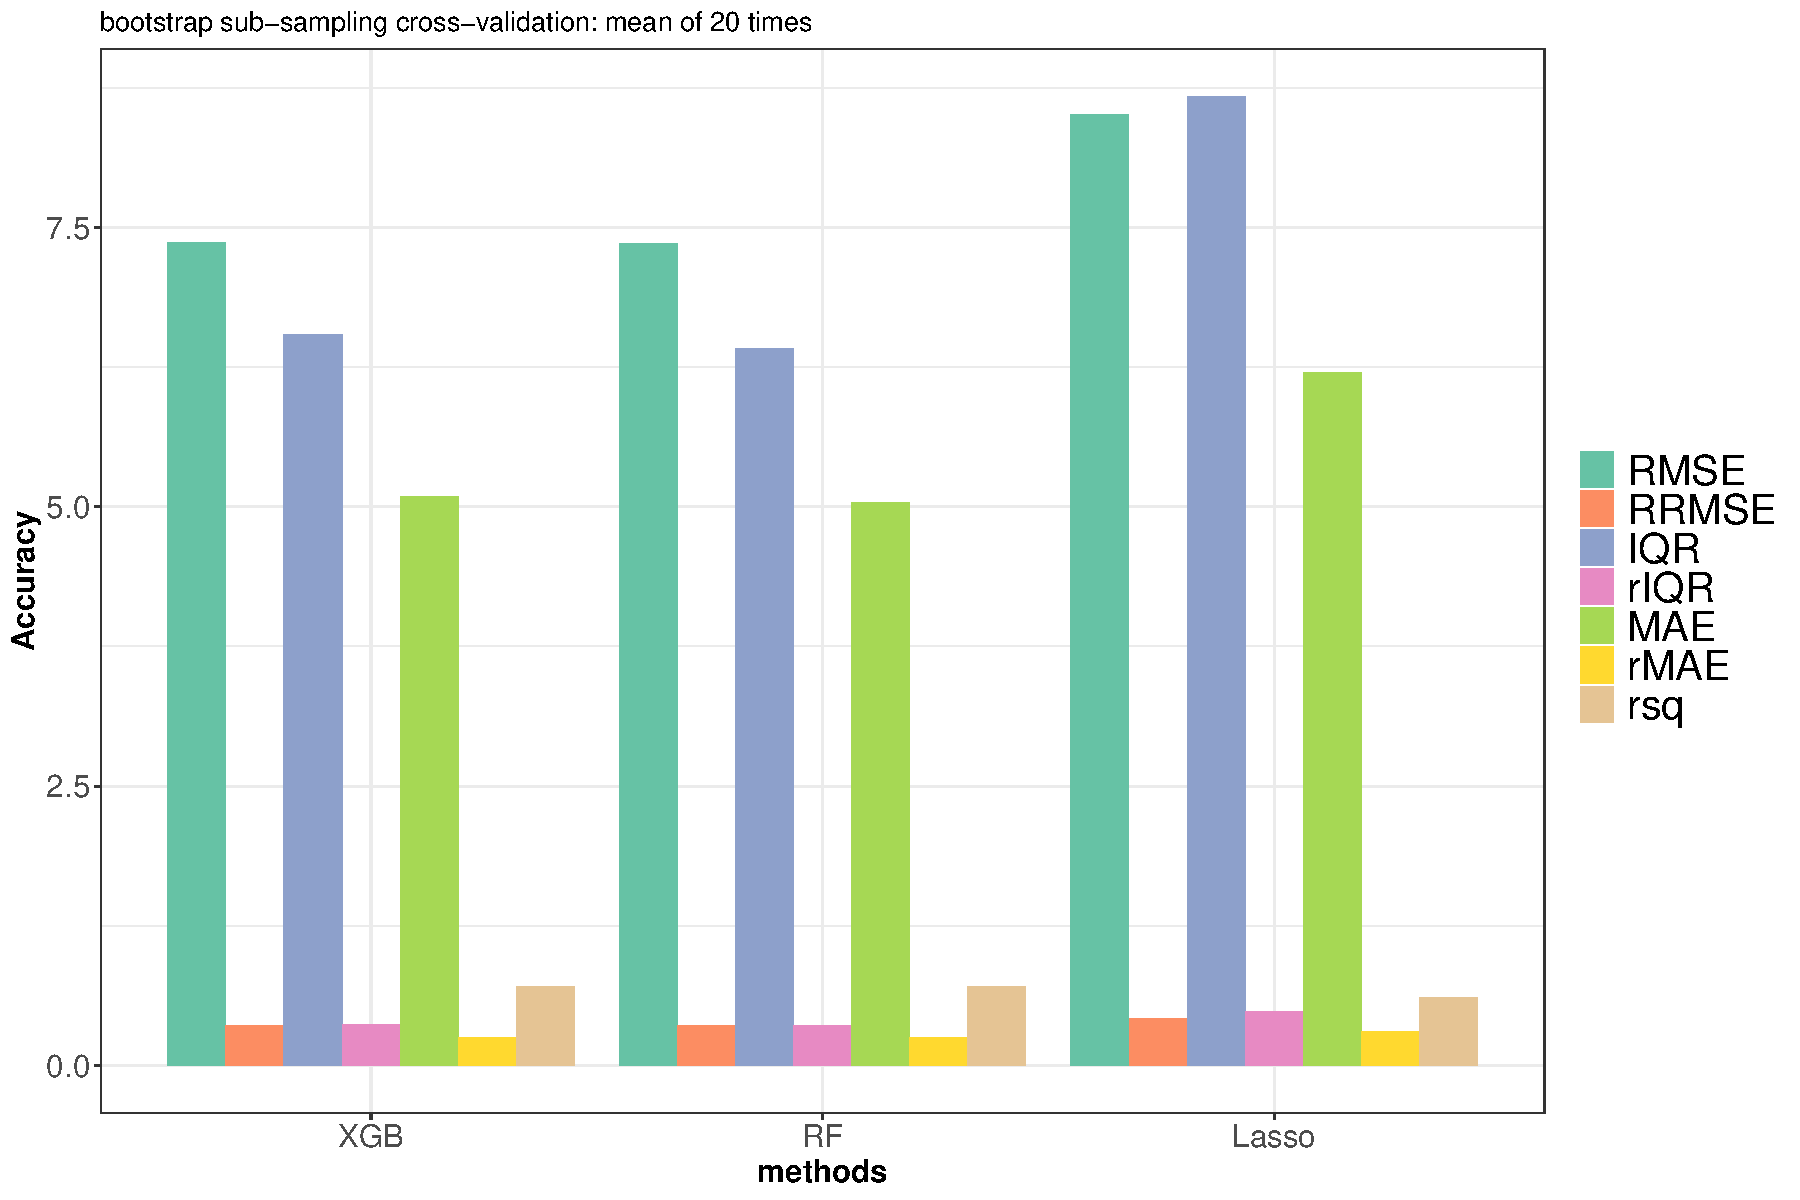
\includegraphics[width=\linewidth]{w1-1.pdf}
    \label{accuracy}
    \caption { Accuracy assessed for NLDE-XGB, NLDE-RF, NLDE-Lasso.}
  \end{figure}
  
\begin{figure}[h!]
    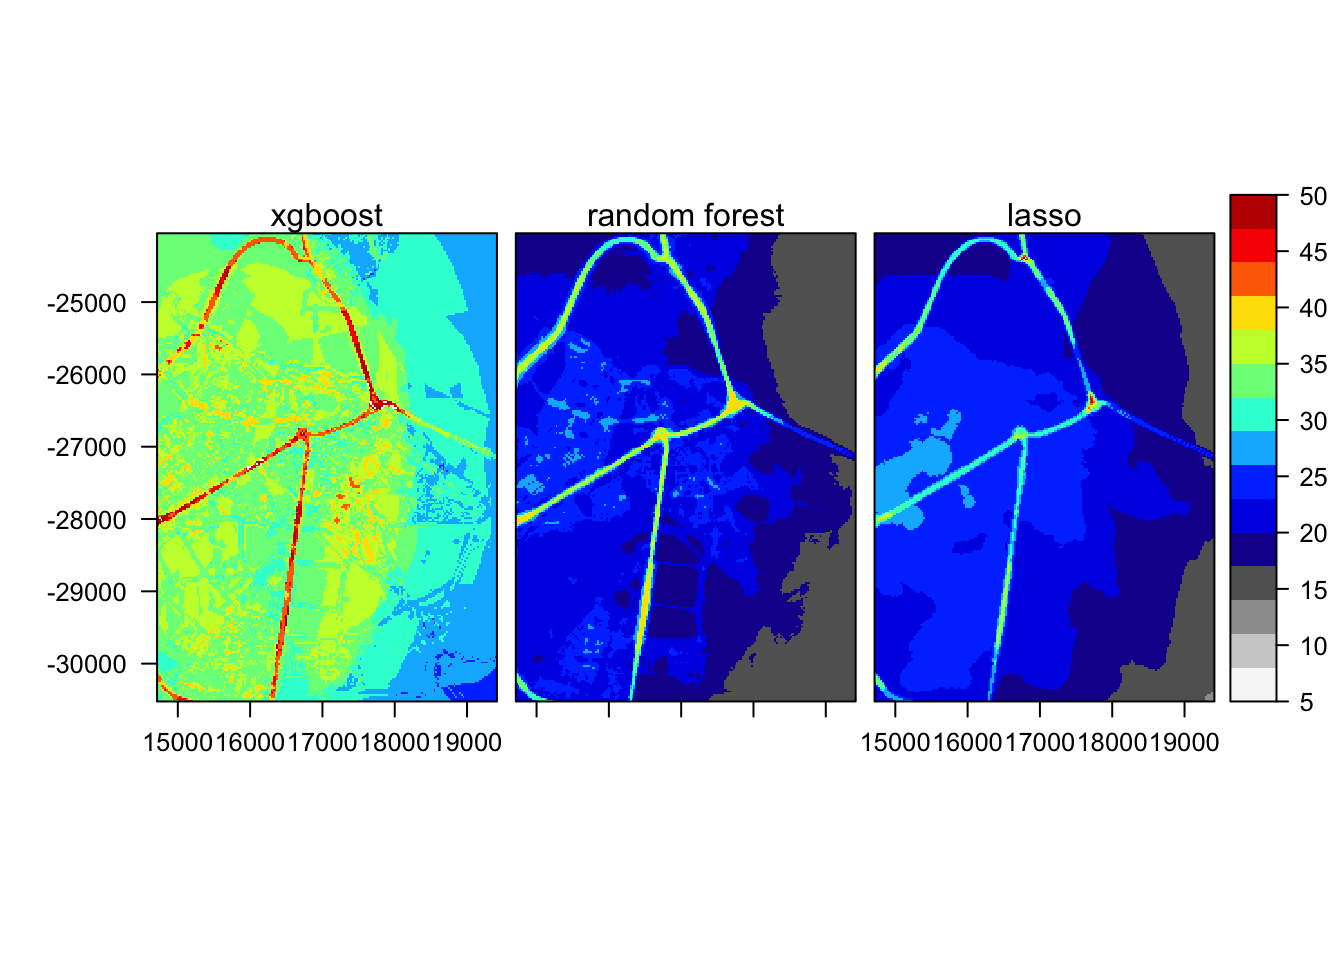
\includegraphics[width=\linewidth]{NLDE.png}
    \label{nldepred}
    \caption {predictions from NLDE-XGB, NLDE-RF, NLDE-Lasso.}
\end{figure}

\subsection{Compare with bakfiets measurements}



\begin{figure}[h!]
    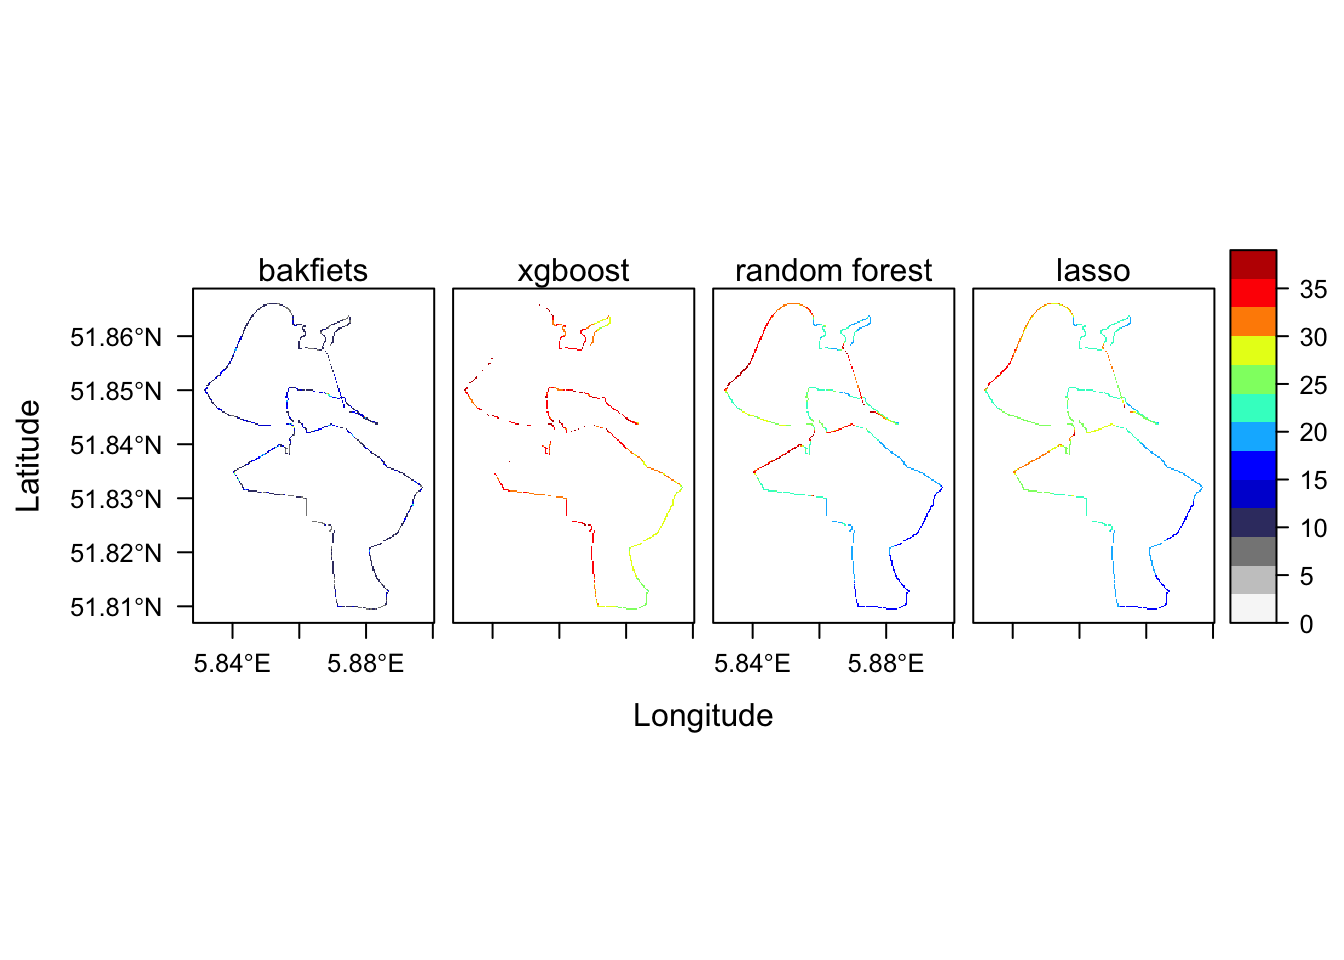
\includegraphics [scale = 0.3 ]{NLDE_vs_bak.png}
    \label{nldevsbak}
    \caption { The differences between NLDE model predictions and cargo-bike measurements, the values are the subtraction of cargo-bike measurements from NLDE model predictions (model prediction - bike measurements), in ug/m3.}
\end{figure}
\subsection{Validation with Cargo-bike measurements}
%pearson correlation coefficient`
 %         xgbnij    rfmnij    Lamnij
%xgbnij 1.0000000 0.7956444 0.7786702
%rfmnij 0.7956444 1.0000000 0.9287154
%Lamnij 0.7786702 0.9287154 1.0000000

%mean
%  xgbnij   rfmnij   Lamnij 
%32.99156 20.67016 21.43969 

\subsection{Global model predictions}
The mean of xgboost, random forest, and Lasso predictions over the area of Nijmegen (called predictions) are respectively 25.77, 22.38, and 26.54 ug/m3. The Nijmegen predictions are shown in figure X. From the figures, the xgboost and random forest predictions reveal more details, they also obtained a higher prediction accuracy (see the global paper) compared to Lasso. Comparing the figure X with the predictors (supplement figure SF2), it can be observed that the predictions reveal primary road patterns. The paired Pearson correlation between three Nijmegen predictions in are: 0.8 for random forest vs. Lasso, 0.81 for random forest vs. xgboost, and 0.94 for Lasso vs. random forest.
\begin{figure}[h!]
    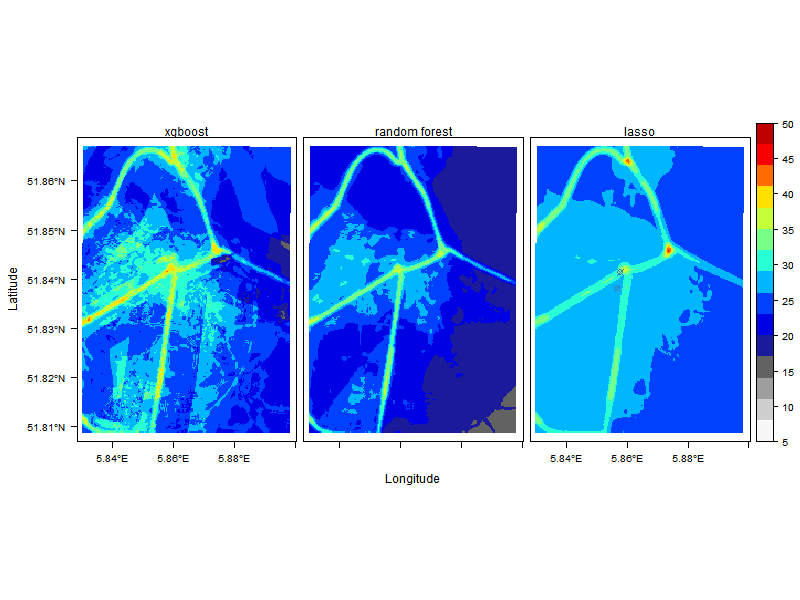
\includegraphics[width=\linewidth]{f3.png}
    \label{seperate}
    \caption {predictions from three global models: xgboost, random forest and lasso. The LML stations that are used in the global model are shown in the Lasso prediction plot.}
\end{figure}
\subsection{Validation with Cargo-bike measurements}

\begin{figure}[h!]
    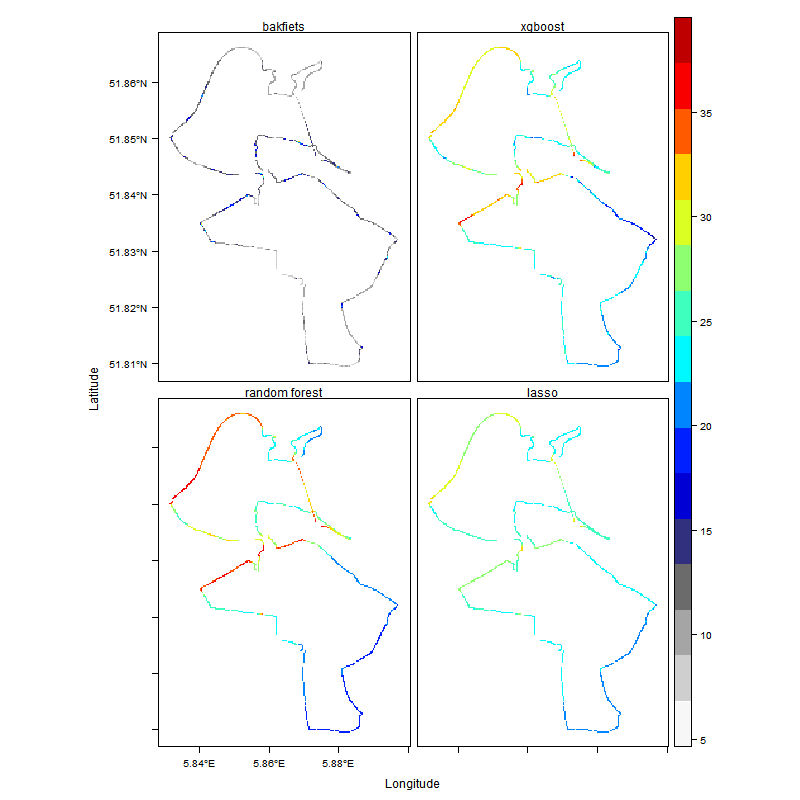
\includegraphics[width=\linewidth]{f4.png}
    \label{seperate}
    \caption {Averaged cargo-bike measurements and global model predictions (scaled). a: scale the cargo-bike using the Graafseweg LML station.}
\end{figure}
The cargo-bike measurements (the distribution is shown in supplementary figure SF1) show higher NO$_2$ in the west and middle, from points 19 -21, 24 -25, and around point 9 (figure 1, called route 19-21, 24-25, and 9), which align well with predictions from the three global models. However, the spatial variations of the cargo-bike measurements are much smaller compared to the global model predictions. The route 19-21 and route 24-25 are estimated much higher by the global models, most notably random forest.    
\par
Figure X shows averaged cargo-bike measurements and scaled global model predictions at the cargo-bike track. It shows the global model predictions are higher in magnitudes, however, remember the mean of the global model prediction is closer to the mean of the LML ground station measurements. 
\begin{figure}[h!]
    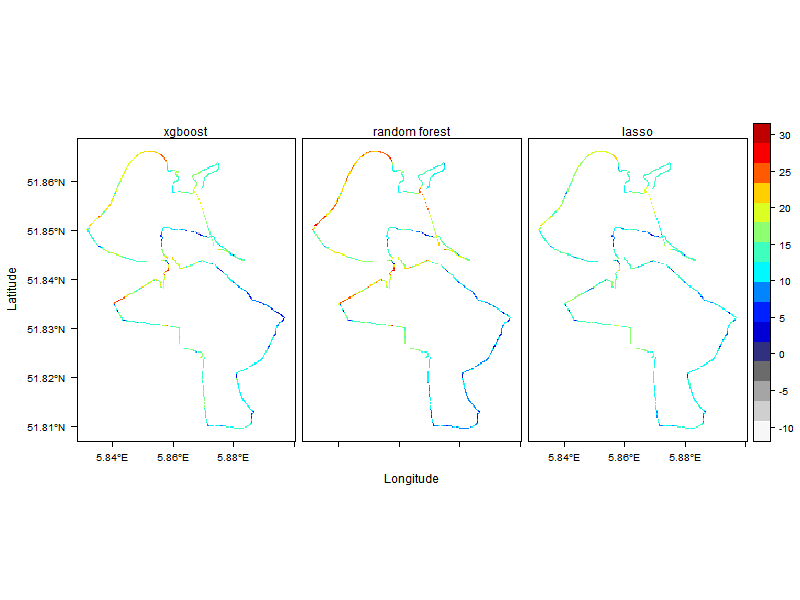
\includegraphics[width=\linewidth]{f4a.png}
    \label{Graafseweg}
    \caption {scale the cargo-bike using the Graafseweg station. The differences between scaled global model predictions and cargo-bike meausrements, the values are the subtraction of cargo-bike measurements from global model predictions (model prediction - bike measurements), in ug/m3.}
\end{figure}
\begin{figure}[h!]
    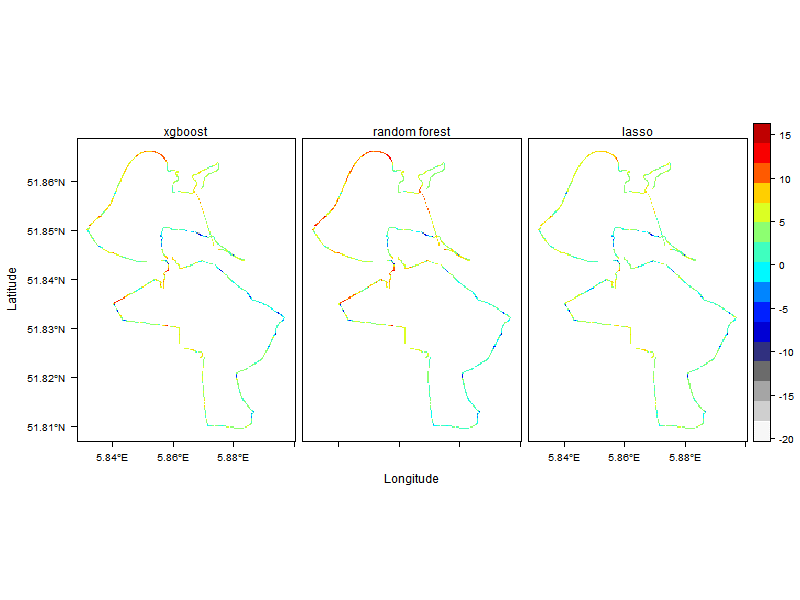
\includegraphics[width=\linewidth]{f4b.png}
    \label{ruyterstraat}
    \caption {scale the cargo-bike using the ruyterstraat station.}
\end{figure}

\bibliography{ref.bib}
\section{Discussion}
\end{document}

https://www.umweltbundesamt.de/en
http://discomap.eea.europa.eu/Index/
